\pdfoutput=1
%% Author: PGL  Porta Mana
%% Created: 2017-10-21T20:53:34+0200
%% Last-Updated: 2019-02-01T14:18:46+0100
%%%%%%%%%%%%%%%%%%%%%%%%%%%%%%%%%%%%%%%%%%%%%%%%%%%%%%%%%%%%%%%%%%%%%%
% Report-no: ***
\newif\ifarxiv
\arxivfalse
\ifarxiv\pdfmapfile{+classico.map}\fi
\newif\ifafour
\afourfalse % true = A4, false = A5
\newif\iftypodisclaim % typographical disclaim on the side
\typodisclaimtrue
\newcommand*{\memfontfamily}{zplx}
\newcommand*{\memfontpack}{newpxtext}
\documentclass[\ifafour a4paper,12pt,\else a5paper,10pt,\fi%extrafontsizes,%
onecolumn,oneside,article,%french,italian,german,swedish,latin,
british%
]{memoir}
\newcommand*{\updated}{\today}
\newcommand*{\firstdraft}{21 October 2017}
\newcommand*{\firstpublished}{***}
\newcommand*{\propertitle}{What and wherefore is a probability model?}
\newcommand*{\pdftitle}{\propertitle}
\newcommand*{\headtitle}{\propertitle}
\newcommand*{\pdfauthor}{P.G.L.  Porta Mana}
\newcommand*{\headauthor}{Luca}
\newcommand*{\reporthead}{}
%%%%%%%%%%%%%%%%%%%%%%%%%%%%%%%%%%%%%%%%%%%%%%%%%%%%%%%%%%%%%%%%%%%%%%%%%%%%
%%%%%%%%%%%%%%%%%%%%%%%%%%%%%%%%%%%%%%%%%%%%%%%%%%%%%%%%%%%%%%%%%%%%%%%%%%%%
%\usepackage{pifont}
%\usepackage{fontawesome}
\usepackage[T1]{fontenc} 
\input{glyphtounicode} \pdfgentounicode=1
\usepackage[utf8]{inputenx}
%\usepackage{newunicodechar}
% \newunicodechar{Ĕ}{\u{E}}
% \newunicodechar{ĕ}{\u{e}}
% \newunicodechar{Ĭ}{\u{I}}
% \newunicodechar{ĭ}{\u{\i}}
% \newunicodechar{Ŏ}{\u{O}}
% \newunicodechar{ŏ}{\u{o}}
% \newunicodechar{Ŭ}{\u{U}}
% \newunicodechar{ŭ}{\u{u}}
% \newunicodechar{Ā}{\=A}
% \newunicodechar{ā}{\=a}
% \newunicodechar{Ē}{\=E}
% \newunicodechar{ē}{\=e}
% \newunicodechar{Ī}{\=I}
% \newunicodechar{ī}{\={\i}}
% \newunicodechar{Ō}{\=O}
% \newunicodechar{ō}{\=o}
% \newunicodechar{Ū}{\=U}
% \newunicodechar{ū}{\=u}
% \newunicodechar{Ȳ}{\=Y}
% \newunicodechar{ȳ}{\=y}

\newcommand*{\bmmax}{0} % reduce number of bold fonts, before bm
\newcommand*{\hmmax}{0} % reduce number of heavy fonts, before bm
\usepackage{textcomp}
\usepackage[normalem]{ulem}
% \makeatletter
% \def\ssout{\bgroup \ULdepth=-.35ex%\UL@setULdepth
%  \markoverwith{\lower\ULdepth\hbox
%    {\kern-.03em\vbox{\hrule width.2em\kern1.2\p@\hrule}\kern-.03em}}%
%  \ULon}
% \makeatother
\usepackage{amsmath}
\usepackage{mathtools}
\addtolength{\jot}{\jot} % increase spacing in multiline formulae
\usepackage{empheq}% automatically calls amsmath and mathtools
\newcommand*{\widefbox}[1]{\fbox{\hspace{1em}#1\hspace{1em}}}
\setlength{\multlinegap}{0pt}
%\usepackage{fancybox}
%\usepackage{framed}
% \usepackage[misc]{ifsym} % for dice
% \newcommand*{\diceone}{{\scriptsize\Cube{1}}}
\usepackage{amssymb}
\usepackage{amsxtra}

\usepackage[main=british,french,italian,german,swedish,latin,esperanto]{babel}\selectlanguage{british}
\newcommand*{\langfrench}{\foreignlanguage{french}}
\newcommand*{\langgerman}{\foreignlanguage{german}}
\newcommand*{\langitalian}{\foreignlanguage{italian}}
\newcommand*{\langswedish}{\foreignlanguage{swedish}}
\newcommand*{\langlatin}{\foreignlanguage{latin}}
\newcommand*{\langnohyph}{\foreignlanguage{nohyphenation}}

\usepackage[autostyle=false,autopunct=false,english=british]{csquotes}
\setquotestyle{british}

\usepackage{amsthm}
\newcommand*{\QED}{\textsc{q.e.d.}}
\renewcommand*{\qedsymbol}{\QED}
\theoremstyle{remark}
\newtheorem{note}{Note}
\newtheorem*{remark}{Note}
\newtheoremstyle{innote}{\parsep}{\parsep}{\footnotesize}{}{}{}{0pt}{}
\theoremstyle{innote}
\newtheorem*{innote}{}


\usepackage[shortlabels,inline]{enumitem}
\SetEnumitemKey{para}{itemindent=\parindent,leftmargin=0pt,listparindent=\parindent,parsep=0pt,itemsep=\topsep}
% \begin{asparaenum} = \begin{enumerate}[para]
% \begin{inparaenum} = \begin{enumerate*}
\setlist[enumerate,2]{label=\alph*.}
\setlist[enumerate]{label=\arabic*.,leftmargin=1.5\parindent}
\setlist[itemize]{leftmargin=1.5\parindent}
\setlist[description]{leftmargin=1.5\parindent}
% old alternative:
% \setlist[enumerate,2]{label=\alph*.}
% \setlist[enumerate]{leftmargin=\parindent}
% \setlist[itemize]{leftmargin=\parindent}
% \setlist[description]{leftmargin=\parindent}

\usepackage[babel,theoremfont,largesc]{newpxtext}
\usepackage[bigdelims,nosymbolsc%,smallerops % probably arXiv doesn't have it
]{newpxmath}
\useosf\linespread{1.083}
%% smaller operators for old version of newpxmath
\makeatletter
\def\re@DeclareMathSymbol#1#2#3#4{%
    \let#1=\undefined
    \DeclareMathSymbol{#1}{#2}{#3}{#4}}
%\re@DeclareMathSymbol{\bigsqcupop}{\mathop}{largesymbols}{"46}
%\re@DeclareMathSymbol{\bigodotop}{\mathop}{largesymbols}{"4A}
\re@DeclareMathSymbol{\bigoplusop}{\mathop}{largesymbols}{"4C}
\re@DeclareMathSymbol{\bigotimesop}{\mathop}{largesymbols}{"4E}
\re@DeclareMathSymbol{\sumop}{\mathop}{largesymbols}{"50}
\re@DeclareMathSymbol{\prodop}{\mathop}{largesymbols}{"51}
\re@DeclareMathSymbol{\bigcupop}{\mathop}{largesymbols}{"53}
\re@DeclareMathSymbol{\bigcapop}{\mathop}{largesymbols}{"54}
%\re@DeclareMathSymbol{\biguplusop}{\mathop}{largesymbols}{"55}
\re@DeclareMathSymbol{\bigwedgeop}{\mathop}{largesymbols}{"56}
\re@DeclareMathSymbol{\bigveeop}{\mathop}{largesymbols}{"57}
%\re@DeclareMathSymbol{\bigcupdotop}{\mathop}{largesymbols}{"DF}
%\re@DeclareMathSymbol{\bigcapplusop}{\mathop}{largesymbolsPXA}{"00}
%\re@DeclareMathSymbol{\bigsqcupplusop}{\mathop}{largesymbolsPXA}{"02}
%\re@DeclareMathSymbol{\bigsqcapplusop}{\mathop}{largesymbolsPXA}{"04}
%\re@DeclareMathSymbol{\bigsqcapop}{\mathop}{largesymbolsPXA}{"06}
\re@DeclareMathSymbol{\bigtimesop}{\mathop}{largesymbolsPXA}{"10}
%\re@DeclareMathSymbol{\coprodop}{\mathop}{largesymbols}{"60}
%\re@DeclareMathSymbol{\varprod}{\mathop}{largesymbolsPXA}{16}
\makeatother


%% With euler font cursive for Greek letters - the [1] means 100% scaling
\DeclareFontFamily{U}{egreek}{\skewchar\font'177}%
\DeclareFontShape{U}{egreek}{m}{n}{<-6>s*[1]eurm5 <6-8>s*[1]eurm7 <8->s*[1]eurm10}{}%
\DeclareFontShape{U}{egreek}{m}{it}{<->s*[1]eurmo10}{}%
\DeclareFontShape{U}{egreek}{b}{n}{<-6>s*[1]eurb5 <6-8>s*[1]eurb7 <8->s*[1]eurb10}{}%
\DeclareFontShape{U}{egreek}{b}{it}{<->s*[1]eurbo10}{}%
\DeclareSymbolFont{egreeki}{U}{egreek}{m}{it}%
\SetSymbolFont{egreeki}{bold}{U}{egreek}{b}{it}% from the amsfonts package
\DeclareSymbolFont{egreekr}{U}{egreek}{m}{n}%
\SetSymbolFont{egreekr}{bold}{U}{egreek}{b}{n}% from the amsfonts package
% Take also \sum, \prod, \coprod symbols from Euler fonts
\DeclareFontFamily{U}{egreekx}{\skewchar\font'177}
\DeclareFontShape{U}{egreekx}{m}{n}{%
       <-7.5>s*[0.9]euex7%
    <7.5-8.5>s*[0.9]euex8%
    <8.5-9.5>s*[0.9]euex9%
    <9.5->s*[0.9]euex10%
}{}
\DeclareSymbolFont{egreekx}{U}{egreekx}{m}{n}
\DeclareMathSymbol{\sumop}{\mathop}{egreekx}{"50}
\DeclareMathSymbol{\prodop}{\mathop}{egreekx}{"51}
\DeclareMathSymbol{\coprodop}{\mathop}{egreekx}{"60}
\makeatletter
\def\sum{\DOTSI\sumop\slimits@}
\def\prod{\DOTSI\prodop\slimits@}
\def\coprod{\DOTSI\coprodop\slimits@}
\makeatother
% Greek letters not usually given in LaTeX.
\DeclareMathSymbol{\varpartial}{\mathalpha}{egreeki}{"40}
\DeclareMathSymbol{\partialup}{\mathalpha}{egreekr}{"40}
\DeclareMathSymbol{\alpha}{\mathalpha}{egreeki}{"0B}
\DeclareMathSymbol{\beta}{\mathalpha}{egreeki}{"0C}
\DeclareMathSymbol{\gamma}{\mathalpha}{egreeki}{"0D}
\DeclareMathSymbol{\delta}{\mathalpha}{egreeki}{"0E}
\DeclareMathSymbol{\epsilon}{\mathalpha}{egreeki}{"0F}
\DeclareMathSymbol{\zeta}{\mathalpha}{egreeki}{"10}
\DeclareMathSymbol{\eta}{\mathalpha}{egreeki}{"11}
\DeclareMathSymbol{\theta}{\mathalpha}{egreeki}{"12}
\DeclareMathSymbol{\iota}{\mathalpha}{egreeki}{"13}
\DeclareMathSymbol{\kappa}{\mathalpha}{egreeki}{"14}
\DeclareMathSymbol{\lambda}{\mathalpha}{egreeki}{"15}
\DeclareMathSymbol{\mu}{\mathalpha}{egreeki}{"16}
\DeclareMathSymbol{\nu}{\mathalpha}{egreeki}{"17}
\DeclareMathSymbol{\xi}{\mathalpha}{egreeki}{"18}
\DeclareMathSymbol{\omicron}{\mathalpha}{egreeki}{"6F}
\DeclareMathSymbol{\pi}{\mathalpha}{egreeki}{"19}
\DeclareMathSymbol{\rho}{\mathalpha}{egreeki}{"1A}
\DeclareMathSymbol{\sigma}{\mathalpha}{egreeki}{"1B}
 \DeclareMathSymbol{\tau}{\mathalpha}{egreeki}{"1C}
\DeclareMathSymbol{\upsilon}{\mathalpha}{egreeki}{"1D}
\DeclareMathSymbol{\phi}{\mathalpha}{egreeki}{"1E}
\DeclareMathSymbol{\chi}{\mathalpha}{egreeki}{"1F}
\DeclareMathSymbol{\psi}{\mathalpha}{egreeki}{"20}
\DeclareMathSymbol{\omega}{\mathalpha}{egreeki}{"21}
\DeclareMathSymbol{\varepsilon}{\mathalpha}{egreeki}{"22}
\DeclareMathSymbol{\vartheta}{\mathalpha}{egreeki}{"23}
\DeclareMathSymbol{\varpi}{\mathalpha}{egreeki}{"24}
\let\varrho\rho 
\let\varsigma\sigma
 \let\varkappa\kappa
\DeclareMathSymbol{\varphi}{\mathalpha}{egreeki}{"27}
%
\DeclareMathSymbol{\varAlpha}{\mathalpha}{egreeki}{"41}
\DeclareMathSymbol{\varBeta}{\mathalpha}{egreeki}{"42}
\DeclareMathSymbol{\varGamma}{\mathalpha}{egreeki}{"00}
\DeclareMathSymbol{\varDelta}{\mathalpha}{egreeki}{"01}
\DeclareMathSymbol{\varEpsilon}{\mathalpha}{egreeki}{"45}
\DeclareMathSymbol{\varZeta}{\mathalpha}{egreeki}{"5A}
\DeclareMathSymbol{\varEta}{\mathalpha}{egreeki}{"48}
\DeclareMathSymbol{\varTheta}{\mathalpha}{egreeki}{"02}
 \DeclareMathSymbol{\varIota}{\mathalpha}{egreeki}{"49}
\DeclareMathSymbol{\varKappa}{\mathalpha}{egreeki}{"4B}
\DeclareMathSymbol{\varLambda}{\mathalpha}{egreeki}{"03}
\DeclareMathSymbol{\varMu}{\mathalpha}{egreeki}{"4D}
\DeclareMathSymbol{\varNu}{\mathalpha}{egreeki}{"4E}
\DeclareMathSymbol{\varXi}{\mathalpha}{egreeki}{"04}
\DeclareMathSymbol{\varOmicron}{\mathalpha}{egreeki}{"4F}
\DeclareMathSymbol{\varPi}{\mathalpha}{egreeki}{"05}
\DeclareMathSymbol{\varRho}{\mathalpha}{egreeki}{"50}
\DeclareMathSymbol{\varSigma}{\mathalpha}{egreeki}{"06}
\DeclareMathSymbol{\varTau}{\mathalpha}{egreeki}{"54}
\DeclareMathSymbol{\varUpsilon}{\mathalpha}{egreeki}{"07}
\DeclareMathSymbol{\varPhi}{\mathalpha}{egreeki}{"08}
\DeclareMathSymbol{\varChi}{\mathalpha}{egreeki}{"58}
\DeclareMathSymbol{\varPsi}{\mathalpha}{egreeki}{"09}
\DeclareMathSymbol{\varOmega}{\mathalpha}{egreeki}{"0A} 
%
\DeclareMathSymbol{\Alpha}{\mathalpha}{egreekr}{"41}
\DeclareMathSymbol{\Beta}{\mathalpha}{egreekr}{"42}
\DeclareMathSymbol{\Gamma}{\mathalpha}{egreekr}{"00}
\DeclareMathSymbol{\Delta}{\mathalpha}{egreekr}{"01}
\DeclareMathSymbol{\Epsilon}{\mathalpha}{egreekr}{"45}
\DeclareMathSymbol{\Zeta}{\mathalpha}{egreekr}{"5A}
\DeclareMathSymbol{\Eta}{\mathalpha}{egreekr}{"48}
\DeclareMathSymbol{\Theta}{\mathalpha}{egreekr}{"02}
\DeclareMathSymbol{\Iota}{\mathalpha}{egreekr}{"49}
\DeclareMathSymbol{\Kappa}{\mathalpha}{egreekr}{"4B}
\DeclareMathSymbol{\Lambda}{\mathalpha}{egreekr}{"03}
\DeclareMathSymbol{\Mu}{\mathalpha}{egreekr}{"4D}
\DeclareMathSymbol{\Nu}{\mathalpha}{egreekr}{"4E}
\DeclareMathSymbol{\Xi}{\mathalpha}{egreekr}{"04}
\DeclareMathSymbol{\Omicron}{\mathalpha}{egreekr}{"4F}
\DeclareMathSymbol{\Pi}{\mathalpha}{egreekr}{"05}
\DeclareMathSymbol{\Rho}{\mathalpha}{egreekr}{"50}
\DeclareMathSymbol{\Sigma}{\mathalpha}{egreekr}{"06}
\DeclareMathSymbol{\Tau}{\mathalpha}{egreekr}{"54}
\DeclareMathSymbol{\Upsilon}{\mathalpha}{egreekr}{"07}
\DeclareMathSymbol{\Phi}{\mathalpha}{egreekr}{"08}
\DeclareMathSymbol{\Chi}{\mathalpha}{egreekr}{"58}
\DeclareMathSymbol{\Psi}{\mathalpha}{egreekr}{"09}
\DeclareMathSymbol{\Omega}{\mathalpha}{egreekr}{"0A}
%
\DeclareMathSymbol{\alphaup}{\mathalpha}{egreekr}{"0B}
\DeclareMathSymbol{\betaup}{\mathalpha}{egreekr}{"0C}
\DeclareMathSymbol{\gammaup}{\mathalpha}{egreekr}{"0D}
 \DeclareMathSymbol{\deltaup}{\mathalpha}{egreekr}{"0E}
\DeclareMathSymbol{\epsilonup}{\mathalpha}{egreekr}{"0F}
\DeclareMathSymbol{\zetaup}{\mathalpha}{egreekr}{"10}
\DeclareMathSymbol{\etaup}{\mathalpha}{egreekr}{"11}
\DeclareMathSymbol{\thetaup}{\mathalpha}{egreekr}{"12}
\DeclareMathSymbol{\iotaup}{\mathalpha}{egreekr}{"13}
\DeclareMathSymbol{\kappaup}{\mathalpha}{egreekr}{"14}
\DeclareMathSymbol{\lambdaup}{\mathalpha}{egreekr}{"15}
\DeclareMathSymbol{\muup}{\mathalpha}{egreekr}{"16}
\DeclareMathSymbol{\nuup}{\mathalpha}{egreekr}{"17}
\DeclareMathSymbol{\xiup}{\mathalpha}{egreekr}{"18}
\DeclareMathSymbol{\omicronup}{\mathalpha}{egreekr}{"6F}
  \DeclareMathSymbol{\piup}{\mathalpha}{egreekr}{"19}
\DeclareMathSymbol{\rhoup}{\mathalpha}{egreekr}{"1A}
\DeclareMathSymbol{\sigmaup}{\mathalpha}{egreekr}{"1B}
\DeclareMathSymbol{\tauup}{\mathalpha}{egreekr}{"1C}
\DeclareMathSymbol{\upsilonup}{\mathalpha}{egreekr}{"1D}
\DeclareMathSymbol{\phiup}{\mathalpha}{egreekr}{"1E}
\DeclareMathSymbol{\chiup}{\mathalpha}{egreekr}{"1F}
\DeclareMathSymbol{\psiup}{\mathalpha}{egreekr}{"20}
\DeclareMathSymbol{\omegaup}{\mathalpha}{egreekr}{"21}
\DeclareMathSymbol{\varepsilonup}{\mathalpha}{egreekr}{"22}
\DeclareMathSymbol{\varthetaup}{\mathalpha}{egreekr}{"23}
\DeclareMathSymbol{\varpiup}{\mathalpha}{egreekr}{"24}
\let\varrhoup\rhoup 
\let\varsigmaup\sigmaup
\let\varkappaup\kappaup
\DeclareMathSymbol{\varphiup}{\mathalpha}{egreekr}{"27}
% Greek letters not usually given in LaTeX.

% Optima as sans-serif font
%\usepackage%[scaled=0.9]%
%{classico}
\renewcommand\sfdefault{uop}
\DeclareMathAlphabet{\mathsf}  {T1}{\sfdefault}{m}{sl}
\SetMathAlphabet{\mathsf}{bold}{T1}{\sfdefault}{b}{sl}
\newcommand*{\mathte}[1]{\textbf{\textit{\textsf{#1}}}}
% Upright sans-serif math alphabet
% \DeclareMathAlphabet{\mathsu}  {T1}{\sfdefault}{m}{n}
% \SetMathAlphabet{\mathsu}{bold}{T1}{\sfdefault}{b}{n}

% DejaVu Mono as typewriter text
\usepackage[scaled=0.84]{DejaVuSansMono}


\usepackage{mathdots}

\usepackage[usenames]{xcolor}
% Tol (2012) colour-blind-, print-, screen-friendly colours, alternative scheme; Munsell terminology
\definecolor{mypurpleblue}{RGB}{68,119,170}
\definecolor{myblue}{RGB}{102,204,238}
\definecolor{mygreen}{RGB}{34,136,51}
\definecolor{myyellow}{RGB}{204,187,68}
\definecolor{myred}{RGB}{238,102,119}
\definecolor{myredpurple}{RGB}{170,51,119}
\definecolor{mygrey}{RGB}{187,187,187}

% Tol (2012) colour-blind-, print-, screen-friendly colours; Munsell terminology
% \definecolor{lbpurple}{RGB}{51,34,136}
% \definecolor{lblue}{RGB}{136,204,238}
% \definecolor{lbgreen}{RGB}{68,170,153}
% \definecolor{lgreen}{RGB}{17,119,51}
% \definecolor{lgyellow}{RGB}{153,153,51}
% \definecolor{lyellow}{RGB}{221,204,119}
% \definecolor{lred}{RGB}{204,102,119}
% \definecolor{lpred}{RGB}{136,34,85}
% \definecolor{lrpurple}{RGB}{170,68,153}
 \definecolor{lgrey}{RGB}{221,221,221}
%\newcommand*\mycolourbox[1]{%
%\colorbox{mygrey}{\hspace{1em}#1\hspace{1em}}}
\colorlet{shadecolor}{lgrey}

\usepackage{bm}
\usepackage{microtype}

\usepackage[backend=biber,mcite,%subentry,
citestyle=authoryear-comp,bibstyle=pglpm-authoryear,autopunct=false,sorting=ny,sortcites=false,natbib=false,maxcitenames=1,maxbibnames=3,minbibnames=1,giveninits=true,uniquename=false,uniquelist=false,maxalphanames=1,block=space,hyperref=true,defernumbers=false,useprefix=true,sortupper=false,language=british,parentracker=false]{biblatex}
\DeclareSortingScheme{ny}{\sort{\field{sortname}\field{author}\field{editor}}\sort{\field{year}}}
\iffalse\makeatletter%%% replace parenthesis with brackets
\newrobustcmd*{\parentexttrack}[1]{%
  \begingroup
  \blx@blxinit
  \blx@setsfcodes
  \blx@bibopenparen#1\blx@bibcloseparen
  \endgroup}
\AtEveryCite{%
  \let\parentext=\parentexttrack%
  \let\bibopenparen=\bibopenbracket%
  \let\bibcloseparen=\bibclosebracket}
\makeatother\fi
\DefineBibliographyExtras{british}{\def\finalandcomma{\addcomma}}
\renewcommand*{\finalnamedelim}{\addcomma\space}
\setcounter{biburlnumpenalty}{1}
\setcounter{biburlucpenalty}{0}
\setcounter{biburllcpenalty}{1}
\DeclareDelimFormat{multicitedelim}{\addsemicolon\space}
\DeclareDelimFormat{compcitedelim}{\addsemicolon\space}
\DeclareDelimFormat{postnotedelim}{\space}
\ifarxiv\else\addbibresource{portamanabib.bib}\fi
\renewcommand{\bibfont}{\footnotesize}
%\appto{\citesetup}{\footnotesize}% smaller font for citations
\defbibheading{bibliography}[\bibname]{\section*{#1}\addcontentsline{toc}{section}{#1}%\markboth{#1}{#1}
}
\newcommand*{\citep}{\parencites}
\newcommand*{\citey}{\parencites*}
%\renewcommand*{\cite}{\parencite}
\renewcommand*{\cites}{\parencites}
\providecommand{\href}[2]{#2}
\providecommand{\eprint}[2]{\texttt{\href{#1}{#2}}}
\newcommand*{\amp}{\&}
% \newcommand*{\citein}[2][]{\textnormal{\textcite[#1]{#2}}%\addtocategory{extras}{#2}
% }
\newcommand*{\citein}[2][]{\textnormal{\textcite[#1]{#2}}%\addtocategory{extras}{#2}
}
\newcommand*{\citebi}[2][]{\textcite[#1]{#2}%\addtocategory{extras}{#2}
}
\newcommand*{\subtitleproc}[1]{}
\newcommand*{\chapb}{ch.}

% \def\arxivp{}
% \def\mparcp{}
% \def\philscip{}
% \def\biorxivp{}
% \newcommand*{\arxivsi}{\texttt{arXiv} eprints available at \url{http://arxiv.org/}.\\}
% \newcommand*{\mparcsi}{\texttt{mp\_arc} eprints available at \url{http://www.ma.utexas.edu/mp_arc/}.\\}
% \newcommand*{\philscisi}{\texttt{philsci} eprints available at \url{http://philsci-archive.pitt.edu/}.\\}
% \newcommand*{\biorxivsi}{\texttt{bioRxiv} eprints available at \url{http://biorxiv.org/}.\\}
\newcommand*{\arxiveprint}[1]{%\global\def\arxivp{\arxivsi}%\citeauthor{0arxivcite}\addtocategory{ifarchcit}{0arxivcite}%eprint
\texttt{\urlalt{https://arxiv.org/abs/#1}{arXiv:\hspace{0pt}#1}}%
%\texttt{\href{http://arxiv.org/abs/#1}{\protect\url{arXiv:#1}}}%
%\renewcommand{\arxivnote}{\texttt{arXiv} eprints available at \url{http://arxiv.org/}.}
}
\newcommand*{\mparceprint}[1]{%\global\def\mparcp{\mparcsi}%\citeauthor{0mparccite}\addtocategory{ifarchcit}{0mparccite}%eprint
\texttt{\urlalt{http://www.ma.utexas.edu/mp_arc-bin/mpa?yn=#1}{mp\_arc:\hspace{0pt}#1}}%
%\texttt{\href{http://www.ma.utexas.edu/mp_arc-bin/mpa?yn=#1}{\protect\url{mp_arc:#1}}}%
%\providecommand{\mparcnote}{\texttt{mp_arc} eprints available at \url{http://www.ma.utexas.edu/mp_arc/}.}
}
\newcommand*{\philscieprint}[1]{%\global\def\philscip{\philscisi}%\citeauthor{0philscicite}\addtocategory{ifarchcit}{0philscicite}%eprint
\texttt{\urlalt{http://philsci-archive.pitt.edu/archive/#1}{PhilSci:\hspace{0pt}#1}}%
%\texttt{\href{http://philsci-archive.pitt.edu/archive/#1}{\protect\url{PhilSci:#1}}}%
%\providecommand{\mparcnote}{\texttt{philsci} eprints available at \url{http://philsci-archive.pitt.edu/}.}
}
\newcommand*{\biorxiveprint}[1]{%\global\def\biorxivp{\biorxivsi}%\citeauthor{0arxivcite}\addtocategory{ifarchcit}{0arxivcite}%eprint
\texttt{\urlalt{https://doi.org/10.1101/#1}{bioRxiv doi:\hspace{0pt}10.1101/#1}}%
%\texttt{\href{http://arxiv.org/abs/#1}{\protect\url{arXiv:#1}}}%
%\renewcommand{\arxivnote}{\texttt{arXiv} eprints available at \url{http://arxiv.org/}.}
}
\newcommand*{\osfeprint}[1]{%
\texttt{\urlalt{https://doi.org/10.17605/osf.io/#1}{Open Science Framework doi:10.17605/osf.io/#1}}%
}

\usepackage{graphicx}
%\usepackage{wrapfig}
%\usepackage{tikz-cd}

\PassOptionsToPackage{hyphens}{url}\usepackage[hypertexnames=false]{hyperref}
\usepackage[depth=4]{bookmark}
\hypersetup{colorlinks=true,bookmarksnumbered,pdfborder={0 0 0.25},citebordercolor={0.2667 0.4667 0.6667},citecolor=mypurpleblue,linkbordercolor={0.6667 0.2 0.4667},linkcolor=myredpurple,urlbordercolor={0.1333 0.5333 0.2},urlcolor=mygreen,breaklinks=true,pdftitle={\pdftitle},pdfauthor={\pdfauthor}}
% \usepackage[vertfit=local]{breakurl}% only for arXiv
\providecommand*{\urlalt}{\href}

%%% Layout. I do not know on which kind of paper the reader will print the
%%% paper on (A4? letter? one-sided? double-sided?). So I choose A5, which
%%% provides a good layout for reading on screen and save paper if printed
%%% two pages per sheet. Average length line is 66 characters and page
%%% numbers are centred.
\ifafour\setstocksize{297mm}{210mm}%{*}% A4
\else\setstocksize{210mm}{5.5in}%{*}% 210x139.7
\fi
\settrimmedsize{\stockheight}{\stockwidth}{*}
\setlxvchars[\normalfont] %313.3632pt for a 66-characters line
\setxlvchars[\normalfont]
\setlength{\trimtop}{0pt}
\setlength{\trimedge}{\stockwidth}
\addtolength{\trimedge}{-\paperwidth}
% The length of the normalsize alphabet is 133.05988pt - 10 pt = 26.1408pc
% The length of the normalsize alphabet is 159.6719pt - 12pt = 30.3586pc
% Bringhurst gives 32pc as boundary optimal with 69 ch per line
% The length of the normalsize alphabet is 191.60612pt - 14pt = 35.8634pc
\ifafour\settypeblocksize{*}{32pc}{1.618} % A4
%\setulmargins{*}{*}{1.667}%gives 5/3 margins % 2 or 1.667
\else\settypeblocksize{*}{26pc}{1.618}% nearer to a 66-line newpx and preserves GR
\fi
\setulmargins{*}{*}{1}%gives equal margins
\setlrmargins{*}{*}{*}
\setheadfoot{\onelineskip}{2.5\onelineskip}
\setheaderspaces{*}{2\onelineskip}{*}
\setmarginnotes{2ex}{10mm}{0pt}
\checkandfixthelayout[nearest]
\fixpdflayout
%%% End layout
%% this fixes missing white spaces
\pdfmapline{+dummy-space <dummy-space.pfb}\pdfinterwordspaceon%

%%% Sectioning
\newcommand*{\asudedication}[1]{%
{\par\centering\textit{#1}\par}}
\newenvironment{acknowledgements}{\section*{Thanks}\addcontentsline{toc}{section}{Thanks}}{\par}
\makeatletter\renewcommand{\appendix}{\par
  \bigskip{\centering
   \interlinepenalty \@M
   \normalfont
   \printchaptertitle{\sffamily\appendixpagename}\par}
  \setcounter{section}{0}%
  \gdef\@chapapp{\appendixname}%
  \gdef\thesection{\@Alph\c@section}%
  \anappendixtrue}\makeatother
\counterwithout{section}{chapter}
\setsecnumformat{\upshape\csname the#1\endcsname\quad}
\setsecheadstyle{\large\bfseries\sffamily%
\raggedright}
\setsubsecheadstyle{\bfseries\sffamily%
\raggedright}
%\setbeforesecskip{-1.5ex plus 1ex minus .2ex}% plus 1ex minus .2ex}
%\setaftersecskip{1.3ex plus .2ex }% plus 1ex minus .2ex}
%\setsubsubsecheadstyle{\bfseries\sffamily\slshape\raggedright}
%\setbeforesubsecskip{1.25ex plus 1ex minus .2ex }% plus 1ex minus .2ex}
%\setaftersubsecskip{-1em}%{-0.5ex plus .2ex}% plus 1ex minus .2ex}
\setsubsecindent{0pt}%0ex plus 1ex minus .2ex}
\setparaheadstyle{\bfseries\sffamily%
\raggedright}
\setcounter{secnumdepth}{2}
\setlength{\headwidth}{\textwidth}
\newcommand{\addchap}[1]{\chapter*[#1]{#1}\addcontentsline{toc}{chapter}{#1}}
\newcommand{\addsec}[1]{\section*{#1}\addcontentsline{toc}{section}{#1}}
\newcommand{\addsubsec}[1]{\subsection*{#1}\addcontentsline{toc}{subsection}{#1}}
\newcommand{\addpara}[1]{\paragraph*{#1.}\addcontentsline{toc}{subsubsection}{#1}}
\newcommand{\addparap}[1]{\paragraph*{#1}\addcontentsline{toc}{subsubsection}{#1}}

% Headers and footers
\copypagestyle{manaart}{plain}
\makeheadrule{manaart}{\headwidth}{0.5\normalrulethickness}
\makeoddhead{manaart}{%
{\footnotesize%\sffamily%
\scshape\headauthor}}{}{{\footnotesize\sffamily%
\headtitle}}
\makeoddfoot{manaart}{}{\thepage}{}
\newcommand*\autanet{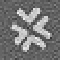
\includegraphics[height=\heightof{M}]{autanet.pdf}}
\definecolor{mygray}{gray}{0.333}
\iftypodisclaim%
\ifafour\newcommand\addprintnote{\begin{picture}(0,0)%
\put(245,149){\makebox(0,0){\rotatebox{90}{\tiny\color{mygray}\textsf{This
            document is designed for screen reading and
            two-up printing on A4 or Letter paper}}}}%
\end{picture}}% A4
\else\newcommand\addprintnote{\begin{picture}(0,0)%
\put(176,112){\makebox(0,0){\rotatebox{90}{\tiny\color{mygray}\textsf{This
            document is designed for screen reading and
            two-up printing on A4 or Letter paper}}}}%
\end{picture}}\fi%afourtrue
\makeoddfoot{plain}{}{\makebox[0pt]{\thepage}\addprintnote}{}
\else
\makeoddfoot{plain}{}{\makebox[0pt]{\thepage}}{}
\fi%typodisclaimtrue
\makeoddhead{plain}{}{}{\footnotesize\reporthead}

% \copypagestyle{manainitial}{plain}
% \makeheadrule{manainitial}{\headwidth}{0.5\normalrulethickness}
% \makeoddhead{manainitial}{%
% \footnotesize\sffamily%
% \scshape\headauthor}{}{\footnotesize\sffamily%
% \headtitle}
% \makeoddfoot{manaart}{}{\thepage}{}

\pagestyle{manaart}

\setlength{\droptitle}{-3.9\onelineskip}
\pretitle{\begin{center}\Large\sffamily%
\bfseries}
\posttitle{\bigskip\end{center}}

\makeatletter\newcommand*{\atf}{
\includegraphics[%trim=1pt 1pt 0pt 0pt,
totalheight=\heightof{@}]{atblack.png}}\makeatother
\providecommand{\affiliation}[1]{\textsl{\textsf{\footnotesize #1}}}
\providecommand{\epost}[1]{\texttt{\footnotesize\textless#1\textgreater}}
\providecommand{\email}[2]{\href{mailto:#1ZZ@#2 ((remove ZZ))}{#1\protect\atf#2}}

\preauthor{\vspace{-0.5\baselineskip}\begin{center}
\normalsize\sffamily%
\lineskip  0.5em}
\postauthor{\par\end{center}}
\predate{\DTMsetdatestyle{mydate}\begin{center}\footnotesize}
\postdate{\end{center}\vspace{-\medskipamount}}
\usepackage[british]{datetime2}
\DTMnewdatestyle{mydate}%
{% definitions
\renewcommand*{\DTMdisplaydate}[4]{%
\number##3\ \DTMenglishmonthname{##2} ##1}%
\renewcommand*{\DTMDisplaydate}{\DTMdisplaydate}%
}
\DTMsetdatestyle{mydate}


\setfloatadjustment{figure}{\footnotesize}
\captiondelim{\quad}
\captionnamefont{\footnotesize\sffamily%
}
\captiontitlefont{\footnotesize}
\firmlists*
\midsloppy

% handling orphan/widow lines, memman.pdf
% \clubpenalty=10000
% \widowpenalty=10000
% \raggedbottom
% Downes, memman.pdf
\clubpenalty=9996
\widowpenalty=9999
\brokenpenalty=4991
\predisplaypenalty=10000
\postdisplaypenalty=1549
\displaywidowpenalty=1602

\selectlanguage{british}\frenchspacing
%%%%%%%%%%%%%%%%%%%%%%%%%%%%%%%%%%%%%%%%%%%%%%%%%%%%%%%%%%%%%%%%%%%%%%%%%%%%
%%%%%%%%%%%%%%%%%%%%%%%%%%%%%%%%%%%%%%%%%%%%%%%%%%%%%%%%%%%%%%%%%%%%%%%%%%%%
%%%% Paper's details %%%%
\title{\propertitle%\\
%  {\large A geometric commentary on maximum-entropy proofs}% ***
}
\author{%
\hspace*{\stretch{1}}%
%% uncomment if additional authors present
% \parbox{0.5\linewidth}%\makebox[0pt][c]%
% {\protect\centering ***\\%
% \footnotesize\epost{\email{***}{***}}}%
% \hspace*{\stretch{1}}%
\parbox{0.5\linewidth}%\makebox[0pt][c]%
{\protect\centering P.G.L.  Porta Mana\\%
\footnotesize\epost{\email{piero.mana}{ntnu.no}}}%
\hspace*{\stretch{1}}%
%\quad\href{https://orcid.org/0000-0002-6070-0784}{\protect
\includegraphics[scale=0.16]{orcid_32x32.png}\textsc{orcid}:0000-0002-6070-0784}%
}

\date{Draft of \today\ (first drafted \firstdraft)}
%\date{\firstpublished; updated \updated}

%@@@@@@@@@@ new macros @@@@@@@@@@
% Common ones - uncomment as needed
%\providecommand{\nequiv}{\not\equiv}
%\providecommand{\coloneqq}{\mathrel{\mathop:}=}
%\providecommand{\eqqcolon}{=\mathrel{\mathop:}}
%\providecommand{\varprod}{\prod}
\newcommand*{\de}{\partialup}%partial diff
\newcommand*{\pu}{\piup}%constant pi
\newcommand*{\delt}{\deltaup}%Kronecker, Dirac
%\newcommand*{\eps}{\varepsilonup}%Levi-Civita, Heaviside
%\newcommand*{\riem}{\zetaup}%Riemann zeta
%\providecommand{\degree}{\textdegree}% degree
%\newcommand*{\celsius}{\textcelsius}% degree Celsius
%\newcommand*{\micro}{\textmu}% degree Celsius
%\newcommand*{\I}{\mathrm{i}}%imaginary unit
%\newcommand*{\e}{\mathrm{e}}%Neper
\newcommand*{\di}{\mathrm{d}}%differential
%\newcommand*{\Di}{\mathrm{D}}%capital differential
%\newcommand*{\planckc}{\hslash}
%\newcommand*{\avogn}{N_{\textrm{A}}}
%\newcommand*{\NN}{\bm{\mathrm{N}}}
%\newcommand*{\ZZ}{\bm{\mathrm{Z}}}
%\newcommand*{\QQ}{\bm{\mathrm{Q}}}
\newcommand*{\RR}{\bm{\mathrm{R}}}
\newcommand*{\CC}{\bm{\mathrm{C}}}
%\newcommand*{\nabl}{\bm{\nabla}}%nabla
%\DeclareMathOperator{\lb}{lb}%base 2 log
%\DeclareMathOperator{\tr}{tr}%trace
%\DeclareMathOperator{\card}{card}%cardinality
%\DeclareMathOperator{\im}{Im}%im part
%\DeclareMathOperator{\re}{Re}%re part
%\DeclareMathOperator{\sgn}{sgn}%signum
%\DeclareMathOperator{\ent}{ent}%integer less or equal to
%\DeclareMathOperator{\Ord}{O}%same order as
%\DeclareMathOperator{\ord}{o}%lower order than
\newcommand*{\incr}{\triangle}%finite increment
\newcommand*{\defd}{\coloneqq}
\newcommand*{\defs}{\eqqcolon}
%\newcommand*{\Land}{\bigwedge}
%\newcommand*{\Lor}{\bigvee}
%\newcommand*{\lland}{\DOTSB\;\land\;}
%\newcommand*{\llor}{\DOTSB\;\lor\;}
%\newcommand*{\limplies}{\mathbin{\Rightarrow}}%implies
%\newcommand*{\suchthat}{\mid}%{\mathpunct{|}}%such that (eg in sets)
%\newcommand*{\bigst}{\mathpunct{\big|}}%such that (eg in sets)
%\newcommand*{\with}{\colon}%with (list of indices)
%\newcommand*{\mul}{\times}%multiplication
%\newcommand*{\inn}{\cdot}%inner product
%\newcommand*{\dotv}{\mathord{\,\cdot\,}}%variable place
%\newcommand*{\comp}{\circ}%composition of functions
%\newcommand*{\con}{\mathbin{:}}%scal prod of tensors
%\newcommand*{\equi}{\sim}%equivalent to 
\renewcommand*{\asymp}{\simeq}%equivalent to 
%\newcommand*{\corr}{\mathrel{\hat{=}}}%corresponds to
%\providecommand{\varparallel}{\ensuremath{\mathbin{/\mkern-7mu/}}}%parallel (tentative symbol)
\renewcommand{\le}{\leqslant}%less or equal
\renewcommand{\ge}{\geqslant}%greater or equal
\DeclarePairedDelimiter\clcl{[}{]}
\DeclarePairedDelimiter\clop{[}{[}
%\DeclarePairedDelimiter\opcl{]}{]}
%\DeclarePairedDelimiter\opop{]}{[}
\DeclarePairedDelimiter\abs{\lvert}{\rvert}
%\DeclarePairedDelimiter\norm{\lVert}{\rVert}
\DeclarePairedDelimiter\set{\{}{\}}
%\DeclareMathOperator{\pr}{P}%probability
\newcommand*{\pf}{\mathrm{p}}%probability
\newcommand*{\p}{\mathrm{P}}%probability
\newcommand*{\E}{\mathrm{E}}
\renewcommand*{\|}{\nonscript\,\vert\nonscript\;\mathopen{}}
\DeclarePairedDelimiterX{\cond}[2]{(}{)}{#1\nonscript\,\delimsize\vert\nonscript\;\mathopen{}#2}
\DeclarePairedDelimiterX{\condt}[2]{[}{]}{#1\nonscript\,\delimsize\vert\nonscript\;\mathopen{}#2}
%\DeclarePairedDelimiterX{\conds}[2]{\{}{\}}{#1\nonscript\,\delimsize\vert\nonscript\;\mathopen{}#2}
%\newcommand*{\tf}{\mathrm{T}}%probability
%\newcommand*{\+}{\lor}
%\renewcommand{\*}{\land}
\newcommand*{\sect}{\S}% Sect.~
\newcommand*{\sects}{\S\S}% Sect.~
\newcommand*{\chap}{ch.}%
\newcommand*{\chaps}{chs}%
\newcommand*{\bref}{ref.}%
\newcommand*{\brefs}{refs}%
%\newcommand*{\fn}{fn}%
\newcommand*{\eqn}{eq.}%
\newcommand*{\eqns}{eqs}%
\newcommand*{\fig}{fig.}%
\newcommand*{\figs}{figs}%
\newcommand*{\vs}{{vs.}}
\newcommand*{\etc}{{etc.}}
\newcommand*{\ie}{{i.e.}}
%\newcommand*{\ca}{{c.}}
\newcommand*{\eg}{{e.g.}}
\newcommand*{\foll}{{ff.}}
%\newcommand*{\viz}{{viz}}
\newcommand*{\cf}{{cf.}}
%\newcommand*{\Cf}{{Cf.}}
%\newcommand*{\vd}{{v.}}
\newcommand*{\etal}{{et al.}}
%\newcommand*{\etsim}{{et sim.}}
%\newcommand*{\ibid}{{ibid.}}
%\newcommand*{\sic}{{sic}}
%\newcommand*{\id}{\mathte{I}}%id matrix
%\newcommand*{\nbd}{\nobreakdash}%
%\newcommand*{\bd}{\hspace{0pt}}%
%\def\hy{-\penalty0\hskip0pt\relax}
%\newcommand*{\labelbis}[1]{\tag*{(\ref{#1})$_\text{r}$}}
%\newcommand*{\mathbox}[2][.8]{\parbox[t]{#1\columnwidth}{#2}}
%\newcommand*{\zerob}[1]{\makebox[0pt][l]{#1}}
\newcommand*{\tprod}{\mathop{\textstyle\prod}\nolimits}
\newcommand*{\tsum}{\mathop{\textstyle\sum}\nolimits}
%\newcommand*{\tint}{\begingroup\textstyle\int\endgroup\nolimits}
%\newcommand*{\tland}{\mathop{\textstyle\bigwedge}\nolimits}
%\newcommand*{\tlor}{\mathop{\textstyle\bigvee}\nolimits}
%\newcommand*{\sprod}{\mathop{\textstyle\prod}}
%\newcommand*{\ssum}{\mathop{\textstyle\sum}}
%\newcommand*{\sint}{\begingroup\textstyle\int\endgroup}
%\newcommand*{\sland}{\mathop{\textstyle\bigwedge}}
%\newcommand*{\slor}{\mathop{\textstyle\bigvee}}
%\newcommand*{\T}{^\intercal}%transpose
%%\newcommand*{\QEM}%{\textnormal{$\Box$}}%{\ding{167}}
%\newcommand*{\qem}{\leavevmode\unskip\penalty9999 \hbox{}\nobreak\hfill
%\quad\hbox{\QEM}}

\definecolor{notecolour}{RGB}{68,170,153}
%\newcommand*{\puzzle}{{\fontencoding{U}\fontfamily{fontawesometwo}\selectfont\symbol{225}}}
\newcommand*{\puzzle}{\maltese}
\newcommand{\mynote}[1]{ {\color{notecolour}\puzzle\ #1}}
%\newcommand*{\widebar}[1]{{\mkern1.5mu\skew{2}\overline{\mkern-1.5mu#1\mkern-1.5mu}\mkern 1.5mu}}

% \newcommand{\explanation}[4][t]{%\setlength{\tabcolsep}{-1ex}
% %\smash{
% \begin{tabular}[#1]{c}#2\\[0.5\jot]\rule{1pt}{#3}\\#4\end{tabular}}%}
 \newcommand*{\ptext}[1]{\text{\small #1}}
%@@@@ Custom macros for this file @@@@
\DeclareMathOperator*{\argsup}{arg\,sup}
\newcommand*{\dob}{degree of belief}
\newcommand*{\dobs}{degrees of belief}

\newcommand*{\yO}[2]{O^{(#1)}_{#2}}
\newcommand*{\yM}{\varMu}
\newcommand*{\ytheta}{\theta^*}

\newcommand*{\yA}{A}
\newcommand*{\yX}{X}
\newcommand*{\yY}{Y}
\newcommand*{\yx}{\bm{x}}
\newcommand*{\yy}{\bm{y}}
\newcommand*{\yI}{\varIota}
\newcommand*{\yD}{D}
\newcommand*{\yg}{G}
\newcommand*{\yHm}{\yM}
\newcommand*{\ym}{\varEta}
\newcommand*{\yE}{E}
\newcommand*{\snp}{\textsc{snp}}
\newcommand*{\yq}{\bm{q}}
% @@@@@@@@@@ new macros end @@@@@@@@@@

\firmlists
\begin{document}
\captiondelim{\quad}\captionnamefont{\footnotesize}\captiontitlefont{\footnotesize}
\selectlanguage{british}\frenchspacing

%%% Title and abstract %%%
\maketitle
\abstractrunin
\abslabeldelim{}
\renewcommand*{\abstractname}{}
\setlength{\absleftindent}{0pt}
\setlength{\absrightindent}{0pt}
\setlength{\abstitleskip}{-\absparindent}
\begin{abstract}\labelsep 0pt%
  \noindent Some notes on model comparison and selection, hypothesis
  testing, parameter estimation, Bayes factors, null hypotheses, and
  related topics.
  \\\noindent\emph{\footnotesize Note: Dear Reader \amp\ Peer, this
    manuscript is being peer-reviewed by you. Thank you.}
% \par%\\[\jot]
% \noindent
% {\footnotesize PACS: ***}\qquad%
% {\footnotesize MSC: ***}%
%\qquad{\footnotesize Keywords: ***}
\end{abstract}

\selectlanguage{british}\frenchspacing
% \asudedication{\small ***}
% \vspace{\bigskipamount}

% \setlength{\epigraphwidth}{.7\columnwidth}
% %\epigraphposition{flushright}
% \epigraphtextposition{flushright}
% %\epigraphsourceposition{flushright}
% \epigraphfontsize{\footnotesize}
% \setlength{\epigraphrule}{0pt}
% %\setlength{\beforeepigraphskip}{0pt}
% %\setlength{\afterepigraphskip}{0pt}
% \epigraph{\emph{text}}{source}

 \setlength{\epigraphwidth}{.5\columnwidth}
% %\epigraphposition{flushright}
 \epigraphtextposition{flushright}
 %\epigraphsourceposition{flushright}
 \epigraphfontsize{\footnotesize}
 \setlength{\epigraphrule}{0pt}
 %\setlength{\beforeepigraphskip}{0pt}
 %\setlength{\afterepigraphskip}{0pt}
 \epigraph{Where do probability models come from?\\ To judge by the resounding
  silence over this question on the part of most statisticians,\\ it seems
  highly embarrassing.}{\citep[p.~220]{dawid1982}}


\section{Summary}
\label{sec:summary}

The literature on statistical modelling reports several issues with Bayes
factors, improper and Jeffreys priors, model averaging, hypothesis testing,
and similar topics, as discussed in the next section. These issues suggest
that, whenever we face a problem involving \enquote{statistical models}, we
should ask:
\begin{enumerate*}[(\arabic*)]
\item Is this an inference problem -- that is, quantification of
  uncertainty -- or a decision problem?
\item What is our uncertainty, ultimately, about?
\item What must we decide about?
\end{enumerate*}

When the problem is purely inferential, the focus in the current literature
is usually on some kind of parameters. But is parameter uncertainty what we
ultimately care about? It seems to me that in the majority of problems what
we want to quantify is our uncertainty about some concrete situation, for
example whether an individual has a particular disease, or the amount of a
particular natural resource in a particular geographic location. Parameters
may enter the mathematical formulation of our uncertainty about such situations,
but they aren't the end goal.

Focus on the parameters, on the other hand, may be important in particular
kinds of decision problems. For example, a software engineer must choose
the specific form of a function that will be used in some application, say,
to convert handwriting to character codes; or the specific form of a
plausibility model to be used in an automated inferential task. Or a
physicist must choose a particular physical theory \citep[a problem
especially considered by][]{jeffreys1931_r1973,jeffreys1939_r1983} among
competing candidates. In such situations the engineer or physicist has to
choose from a manifold of possible functions or models, and the parameters
are just coordinates on that manifold. Choosing a parameter corresponds to
choosing a function or a model. This kind of problems requires not only a
quantified uncertainty about some \enquote{true} model (a notion to be
thoroughly discussed) but also a quantified gain or loss function for the
final choice. A lot of attention is usually given to the quantification of
uncertainty -- choosing priors, likelihoods, and so on -- but very little
to a reasonable quantification of the gain function. Thus the final quality
of the solution, which involves the product of the two, is poor.

In either case there seems to be a more general problem upstream: the
initial inferential or decision problem is poorly formulated. For example,
many \enquote{null hypothesis} questions force an unnatural dichotomous
view on situations better viewed as a continuum of cases. And many concrete
problems are transformed into metaphysical questions such as \enquote{Is this
  statistical model true?}. This metaphysics is often hidden behind
technical terms, but metaphysics it remains nonetheless.
% baffle comprehension if we
% sit down and try to explain -- without circularly using technical jargon --
% what they're actually asking.

The bottom problem is, in my opinion, that even though formal Bayesian
methods are becoming more common, our way of thinking about and formulating
inference and decision problems is still centred on old recipes. This is
particularly true of the \enquote{null hypothesis}, the \enquote{what is
  the true model}, and the \enquote{what is the true parameter value} ways of
thinking. This kind of initial mismatch between a young method and old
formulations is common in the history of science
\citep{truesdell1968,kline1980_r1982,brush1976c_r1986,brush1976d_r1999,whittaker1910_r1951,whittaker1953}.

Here's a simple example. In genome association studies we observe that some
diseases are more frequent among individuals that carry particular variants
of pieces of \textsc{dna}, called Single-Nucleotide Polymorphisms. This
means that we could examine a person's \snp s to make better guesses on
whether that person has or will develop a particular disease. Our
uncertainty stems from the small size of our samples: we'd like to guess
what the frequencies of the disease conditional the \snp\ variants are in
the full population. Many studies face this kind of question in a
dichotomous way: \enquote{Is this particular \snp\ associated with that
  disease? yes or no?}. % A first problem with this question is the vague
% term \enquote{association} (this vagueness doesn't disappear just because
% we use technical terms like \enquote{linkage}). But, whatever we might
% mean,
But the problem is clearly not dichotomous: there is a continuum of
differences between the frequencies of the disease conditional on the
variants of all \snp s. If we approach the problem more concretely we may
ask: what do we want to use this statistical knowledge for? what choices do
we need to make for that purpose? Suppose that the idea is to build an
automated procedure to examine a person's \snp s in order to diagnose the
disease. However, the cost and time involved allows for the automated check
of, say, only one \snp\ per individual. Our decision problem is to choose
the \snp\ to be used in this automated diagnostics. Assume for simplicity
that the candidate \snp s have only two variants each. The gain in using a
particular \snp\ for diagnostics is proportional to the absolute difference
$\abs{\incr f} \in \clcl{0,1}$ between the frequencies, in the full
population, of the disease conditional on the two variants of that \snp. If
$\abs{\incr f} = 0$ the \snp\ doesn't give any information about the
presence of the disease; if $\abs{\incr f} = 1$ it is a perfect,
deterministic predictor. Let's say that a good gain function is
$\abs{\incr f}^2$. From a sample study with with data $\yD$ and background
information $\yI$, our \dob\ about the differences $\abs{\incr f_i}$ of
some candidates \snp s is
$\pf\cond[\big]{\abs{\incr f_1}, \abs{\incr f_2}, \dotsc}{\yD, \yI}$. Then,
according to decision theory, we should choose that \snp\ $i$ for which the
expectation $\E\cond[\big]{\abs{\incr f_i}^2}{\yD, \yI}$ is highest.


No \enquote{null hypotheses} or dichotomous questions were necessary for
our inference and decision in the simple example above. I believe that this
is the case for many, more complex problems that are today stated in
\enquote{null hypothesis} terms; see for example those examined by Kass
\amp\ Raftery \citey[\sect~2]{kassetal1995}. They only require a change in
perspective.

\bigskip

When a statistical problem is approached from a more concrete and
decisional perspective, our final inferences concern concrete quantities,
and only one probabilistic model is present: the one representing our
uncertainty about those quantities. The model $\yM$ may assume a hierarchic form
with a combination of discrete and continuum parts, for example
\begin{equation}
  \label{eq:example_model_mixed}
  \pf(\yD \| \yM) =
 \sum_i \int\!\di\theta_i\; \pf(\yD \| i, \theta_i,\yM)\;
  \pf(i, \theta_i \| \yM),
\end{equation}
where the continuum parameters $\set{\theta_i}$ may have differing
dimensions. From this point of view model comparison doesn't formally
arise, although the usual and necessary problem of specifying a sensible
prior $\pf(\yD \| i, \theta_i,\yM)$ of course remains. The parameter
posterior given data $\yD$ is
\begin{equation}
  \label{eq:param_posterior_model_mixed}
  \pf(i, \theta_i \| \yD, \yM) =
  \frac{\pf(\yD \| i, \theta_i,\yM)\;  \pf(i, \theta_i \| \yM)
  }{
 \sum_j \int\!\di\theta_j\; \pf(\yD \| j, \theta_j,\yM)\;
  \pf(j, \theta_j \| \yM)
  }.
\end{equation}
If for a specific $k$ we have that
$\int\!\di\theta_k\; \pf(\yD \| k, \theta_k,\yM)\; \pf(k, \theta_k \| \yM)
\to 0$, as it happens for improper priors, then the $(k,\theta_k)$ part
disappears in the two equations above; this indicates that we have used a
silly prior $\pf(\yD \| i, \theta_i,\yM)$.




\mynote{Discussion on whether \enquote{hypotheses} in statistical modelling
are really such, au pair with physical hypotheses. Consider the problem of
the urn with unknown proportion of marbles, though!}

\mynote{The consequence of the purely \enquote{syntactic} calculation and
  update of plausibilities}

Many inference problems boil down to guessing what the next outcome in a
possibly unlimited sequence of observations will be, given the outcomes of
some of the observations in this sequence. If we believe that the precise
order of these outcomes is irrelevant for our guesses (an exchangeability
assumption), then we can break our guess as follows:
\begin{enumerate*}[(\alph*)]
\item\label{item:guess_given_freqs}what would our guess be if we knew the
  relative frequencies of the outcomes in the whole (observed an
  unobserved) sequence?
\item\label{item:guess_freqs}what is our guess about such relative frequencies?
\end{enumerate*}
If the number of observations is very large, by symmetry our
\dob~\ref{item:guess_given_freqs} about the next outcome would be its known
relative frequency. So the remaining guess is~\ref{item:guess_freqs}.
Most inferences about \enquote{true models} can be interpreted as
inferences about the unknown final relative frequencies. This point of view
calls for a leap of imagination about future observations. But the combined
lifespan of the humans involved in our original inference problem is surely
finite, so the number of observations is finite although large. The problem
thus becomes analogous to drawing from a finite urn without replacement,
with the complication that the number of balls in the urn is unknown: a
mixture of generalized hypergeometric distributions. It would be
interesting to prove that the resulting \dob~\ref{item:guess_given_freqs}
from such a mixture can be well approximated by the final relative
frequencies, if our \dob\ about the number of balls is peaked at large
values. I like this pragmatic point of view because it gives concrete sense
to statements about \enquote{true models} but it doesn't call for more
metaphysics than there is in, say, planning what to do in case of sunshine or of
rain tomorrow. And it doesn't bring \enquote{propensities} or other
doubtful physical notions into the picture.


\section{Philosophical points and choices}
\label{sec:philosophy}

It isn't possible to clarify probabilistic modelling without taking a
philosophical stance about matters like reality and uncertainty,
propensity, and similar. Any practitioner is implicitly or explicitly
taking a particular stance.

People believing in propensities think of a probabilistic model as
describing a physical property of the objects observed. This stance has
several problems; most important the fact that as our information about the
objects observed change, so changes the \enquote{propensity}, which
therefore doesn't appear to be a physical property after all. The only
exception are \enquote{delta} (or deterministic or singular) belief
distributions, which cannot change with conditionalization on further
information.

This difference is in fact reflected in the update process. Imagine we have
$N$ observations (or measurements), each with $M$ possible outcomes. We
have $M^N$ possible sequences or \enquote{states of affairs}. Let the
proposition $S_m$ denote that the $m$th sequence occurs (they may be
labelled in $M$-ary notation). Let the proposition $\yO{n}{i}$ denote that
the $i$th outcome occurs at the $n$th observation. We can call each
sequence a \enquote{word}, and an observation a \enquote{letter}. If we
know which word $S_m$ is the case, then the letter at position $n$ is given
by a function $r(n,m)$. Our \dob\ is zero or one:
\begin{equation}
  \label{eq:letter_from_word}
  \pf(\yO{n}{i} \| S_m, \yI) = \delt[i - r(n,m)].
\end{equation}

In a general situation of uncertainty $\yM$ we have a \dob\ about all
possible words, $\pf(S_m \| \yM, \yI)$. Our uncertainty about the outcome
of a measurement is therefore
\begin{equation}
  \label{eq:uncertainty_meas_from_seq}
  \pf(\yO{n}{i} \| \yM, \yI) =
  \sum_m \pf(S_m \| \yM, \yI)\; \pf(\yO{n}{i} \| S_m, \yI)
\end{equation}
Given data $\yD \defd \set{\yO{n_k}{i_k}}$, our \dob\ about the words
updates to
\begin{equation}
  \label{eq:update_dob_words}
  \pf(S_m \| \yD, \yM, \yI) \propto
  \pf(S_m \| \yM, \yI)\;
  \prod_k \pf(\yO{n_k}{i_k} \| S_m, \yI).
\end{equation}
The effect of this update is to confine our belief distribution about $S_m$
to increasingly lower-dimensional faces of the simplex $\set{S_m}$. The
Shannon entropy of our distributions is decreasing. In the end we arrive at
a delta distribution centred on a specific $S_m$.

This \enquote{update motion} toward belief distributions with lower entropy
affects also the belief distributions that had an initial support smaller
than $\set{S_m}$.

In the context just presented we may call \enquote{model} any assumption
$\yM$ that yields a specific belief distribution $\pf(S_m) \|\yM, \yI$ for
the possible words.

An exchangeable model $\yE$ is a special case where we assign equal beliefs
to all words having the same relative frequencies $\yq \defd (q_i)$ of
occurrence of the letters $\set{i}$. Let's denote \enquote{$m \in \yq$} the
fact that the $m$th word has frequencies $\yq$. Then
\begin{equation}
  \label{eq:freq_words_exchang}
  \pf(S_m \| \yE, \yI) =
  \sum_{\yq}\delt(m \in \yq)\; \binom{N!}{(N\yq)!}^{-1}\; \pf(\yq \| \yE, \yI),
\end{equation}
where $\binom{N!}{(N\yq)!}$ is the multinomial coefficient. The fact that
updates move our belief about $\set{S_m}$ towards increasingly
lower-dimensional faces of the simplex is reflected in the fact that our
\dob\ $\pf(\yq \| \yE, \yI)$ about the frequencies gets more and more
concentrated on a specific set of frequencies $\yq$. (If the length $N$ of
the sequences is vastly larger than any about of data we consider, then
oscillating behaviours may occur, of course.)

If $\pf(\yq \| \yE, \yI)$ has support on a lower-dimensional subset of
$\set{\yq}$, the update motion toward the vertices of $\set{S_m}$ is
reflected in the fact that ***\mynote{recheck this argument}

\section{Motivation}
\label{sec:motivation}

The Bayesian literature on probabilistic modelling, including model
comparison, hypothesis testing, and parameter estimation, often considers
exchangeable parametric models for our \dobs, of this form:
\begin{equation}
  \label{eq:example_model_literature}
  \pf(\yD \| \yHm, \yI) =
  \int\!\di\theta\; \pf(\yD \| \theta,\yHm,\yI)\;
  \pf(\theta \| \yHm, \yI),
\end{equation}
where $\yHm$ represents the model, $\yI$ other background information and
assumptions, $\yD$ a sequence of data, and $\theta$ a parameter with values
in some manifold. This is a particular case of an exchangeable model
\citep[\chap~4]{bernardoetal1994_r2000}. \emph{Bayes factors} and
\emph{evidence} \citep{good1985,mackay1992,kass1993,kassetal1995}, and
model averaging
\citep{draper1993_r2005,chatfield1995,draper1995,hoetingetal1999} are often
discussed in this kind of literature. If we have several mutually exclusive
and exhaustive models $\yHm_1$, $\yHm_2$, \dots\ our \dob\ about each given
some data is
\begin{equation}
  \label{eq:plaus_model}
  \pf(\yHm_j \| \yD, \yI) =
  \frac{
  \pf(\yD \| \yHm_j, \yI)\; \pf(\yHm_j \| \yI)
  }{
  \sum_k \pf(\yD \| \yHm_k, \yI)\; \pf(\yHm_k \| \yI)
  };
\end{equation}
this \dob\ involves the \emph{evidence}, which is just
$\pf(\yD \| \yHm_j, \yI)$, \eqn~\eqref{eq:example_model_literature}. The
Bayes factor between two models is just the ratio of their evidences.

The literature reports several open issues in \enquote{model comparison}
and the evaluation of evidences and Bayes factors. For example, to
calculate a model's evidence we must solve the integral in
\eqn~\eqref{eq:example_model_literature}, and this requires specifying a
distribution for the parameters $\pf(\theta \| \yHm, \yI)$. When this
distribution is improper the evidence vanishes, so the ratio of two
evidences becomes undetermined. Several ways of fixing this issue have been
proposed in the literature
\citep{kassetal1995,ohagan1995,bergeretal1996,desantisetal1997,bergeretal1998}.
It has also been pointed out if we choose just one out of several possible
models, basing our choice on their evidence, and then we this model to make
inferences, we can end up misrepresenting our \dob\
\citep{draper1993_r2005,chatfield1995,draper1995,hoetingetal1999}. Our
\dob\ is in fact the weighted average of those given by each model. Yet, in
some concrete applications -- think about the use of a neural net -- we
have to choose only one model. \mynote{some reference justly stated that
  this is the domain of decision theory; can't find it}

These issues invite us to re-examine what we're actually doing in
\enquote{model comparison} or \enquote{model selection}. This is the
purpose of the present note.


\bigskip

From a Bayesian point of view model comparison doesn't really exist or is
superfluous, because if we are unsure about several models $\yHm_j$, then
our \dob, by the theorem of total probability, is just
\begin{equation}
  \label{eq:combined_dob}
  \pf(\yD \| \yI) =
  \sum_j \pf(\yD \| \yHm_j,\yI)\; \pf(\yHm_j \| \yI).
\end{equation}
As we gather new data $\yD'$ our \dob\ is updated to
\begin{equation}
  \label{eq:combined_dob_update}
  \pf(\yD \|\yD', \yI) =
  \frac{\pf(\yD, \yD'\| \yI)}{\pf(\yD' \| \yI)} \equiv
  \frac{\sum_j \pf(\yD, \yD' \| \yHm_j,\yI)\; \pf(\yHm_j \| \yI)}{
    \sum_k \pf(\yD' \| \yHm_k,\yI)\; \pf(\yHm_k \| \yI)},
\end{equation}
which can be suggestively rearranged as follows, multiplying and
dividing by $\pf(\yD' \| \yHm_j, \yI)$:
\begin{equation}
  \label{eq:combined_dob_update_suggestive}
  \pf(\yD \|\yD', \yI) =
  \sum_j
  \underbrace{\frac{\pf(\yD, \yD' \| \yHm_j,\yI)}{\pf(\yD' \| \yHm_j,\yI)}}_{{}\defs\pf(\yD \| \yD', \yHm_j,\yI)}\;
  \underbrace{\frac{
  \pf(\yD' \| \yHm_j, \yI)\; \pf(\yHm_j \| \yI)
  }{
  \sum_k \pf(\yD' \| \yHm_k, \yI)\; \pf(\yHm_k \| \yI)
  }}_{{}\defs\pf(\yHm_j \| \yD', \yI)}.
\end{equation}
This is a weighted sum of our \dobs\ conditional on each model, the weights
being our updated \dobs\ about the model themselves. The models which have
very low updated \dobs\ effectively drop out of the sum, so the probability
calculus is automatically doing \enquote{model selection} for us. From this
point of view, the practice of model selection can be viewed as an
approximation of the formula above. The problem with improper distributions
for the parameters still remains, though: models involving such
distributions assign a vanishing \dob\ to the data and therefore disappear
from \eqns~\eqref{eq:combined_dob_update} and
\eqref{eq:combined_dob_update_suggestive}. We'll discuss this issue later.

If we compare the model-averaging formula~\eqref{eq:combined_dob} with the
parametric formula~\eqref{eq:example_model_literature} for a specific
model, we see that the two have the same structure. The second is just the
continuum limit of the first. In fact many of the issues about model
comparison just discussed appear also when we consider just one model of
parametric form~\eqref{eq:example_model_literature}. Given new gathered
data $\yD'$, our \dob\ is updated to
\begin{equation}
  \label{eq:param_combined_dob_update}
  \pf(\yD \|\yD', \yHm, \yI) =
  \frac{\pf(\yD, \yD'\| \yHm, \yI)}{\pf(\yD' \| \yHm, \yI)} \equiv
  \frac{\int\!\di\theta\; \pf(\yD, \yD' \| \theta, \yHm,\yI)\;
    \pf(\theta \| \yHm, \yI)
  }{
    \int\!\di\theta'\; \pf(\yD' \| \theta',\yHm,\yI)\; \pf(\theta' \|\yHm, \yI)},
\end{equation}
which can be suggestively rearranged as follows, multiplying and
dividing by $\pf(\yD' \|\theta, \yHm, \yI)$:
\begin{multline}
  \label{eq:param_combined_dob_update_suggestive}
  \pf(\yD \|\yD', \yHm, \yI) ={}\\
  \int\!\di\theta\;
  \underbrace{\frac{\pf(\yD, \yD' \|\theta, \yHm,\yI)
    }{
      \pf(\yD' \| \theta, \yHm,\yI)}}_{{}\defs\pf(\yD \| \yD',\theta, \yHm,\yI)}\;
  \underbrace{\frac{
  \pf(\yD' \| \theta, \yHm, \yI)\; \pf(\theta \|\yHm, \yI)
  }{
  \int\!\di\theta'\; \pf(\yD' \| \theta', \yHm, \yI)\; \pf(\theta' \|\yHm, \yI)
  }}_{{}\defs\pf(\theta\|\yD', \yHm, \yI)}.
\end{multline}
This is again equivalent to the model-average
case~\eqref{eq:combined_dob_update_suggestive} but for one important
difference: in the first fraction in the product above, the dependence on
data $\yD'$ disappear:
\begin{equation}
  \label{eq:disappearance_data_given_param}
  \pf(\yD \| \yD',\theta, \yHm,\yI) =
  \pf(\yD \| \theta, \yHm,\yI).
\end{equation}
This is a typical property of parametric models: the presence of the
parameters in the conditional makes all other new data in the conditional
\emph{irrelevant}. Use of an improper distribution
$\pf(\theta \|\yHm, \yI)$ for the parameter usually doesn't lead to
problems in this case if correctly used -- that is, taking the limit only
at the very end of all calculations \citep[\chap~15]{jaynes1994_r2003}.
Analogously to the model-average case, parameters with low updated density
$\pf(\theta \|\yD', \yHm, \yI)$ give a vanishing contribution to the
continuum average~\eqref{eq:param_combined_dob_update_suggestive}, so the
probability calculus is automatically doing a \enquote{parameter selection}
for us. From this point of view, the practice of selecting just one
parameter can be viewed as an approximation of the formula above (though
such approximation can be bad if the density for $\theta$ has many modes).

\medskip

In some situations, however, we can't or don't want to consider all models
in the model-average case~\eqref{eq:combined_dob_update_suggestive}, even
when no model dominates our updated \dob\ over the others. We want just one
model. Similarly, in some situations we can't or don't want to consider all
parameters in the single-model
case~\eqref{eq:param_combined_dob_update_suggestive}, even when the updated
density for the parameter has no dominating peaks. We want just one
parameter. These analogous situations involve \emph{decision theory}, and
therefore require us to assign gain/loss functions. But what is our
decision actually about? is it really about a model or a parameter? or
rather about possible data outcomes? Let's examine these question after
making some remarks on models in general.


\section{Remarks on models}
\label{sec:tentative_def}

I consider exchangeable models, but the following remarks may apply to more
general cases.

Let's use this restricted definition: given a set $\yY$ of possible data,
and possibly a set $\yX$ of conditional data, a \emph{probability model} is
a conjunction $\yM$ of assumptions or hypotheses that allows us to assign a
definite, numerical plausibility
\begin{equation}
  \pf(y_1, y_2,\dotsc \| x_1, x_2, \dotsc, \yM, \yI)
  \label{eq:plaus}
\end{equation}
for every meaningful combination of $y_i \in \yY$ and $x_i \in \yX$. For
the moment I consider finite sets.

This definition applies in particular to exchangeable models, where $\yX$
is empty; to partially exchangeable models, where $\yX$ is a set of labels
for the exchangeable categories; and to models used in machine learning and
neural nets. This definition also include functions or maps
$f \colon \yX \to \yY$ as special cases, when the plausibility is unity for
a particular $y$ only, dependent on $x$:
$\pf(y \| x, \yM, \yI) = \delt[y, f(x)]$.

An important distinction can be made between two kinds of model:
\emph{learning} models and \emph{non-learning} models, which can also be
called \emph{extremal} for reasons explained later.

A learning model $\yM$ is one that yields different plausibilities about
some data $(y_1, y_2, \dotsc) \defs \yy$ conditional on
$(x_1, x_2, \dotsc) \defs \yx$ if we condition on knowledge about other
data $(y_1', y_2', \dotsc) \defs \yy'$, $(x_1', x_2', \dotsc) \defs \yx'$:
\begin{equation}
  \label{eq:learning_def}
  \pf(\yy  \| \yx,\, \yy', \yx',\, \yM, \yI) \ne
  \pf(\yy  \| \yx,\, \yM, \yI).
\end{equation}

A non-learning model is one for which these plausibilities are not affected:
\begin{equation}
  \label{eq:non-learning_def}
  \pf(\yy  \| \yx,\, \yy', \yx',\, \yM, \yI) =
  \pf(\yy  \| \yx,\, \yM, \yI).
\end{equation}
This means that 
\begin{equation}
  \label{eq:non-learning_indep}
  \pf(\yy  \| \yx,\, \yM, \yI) = \prod_i  \pf(y_i \| x_i,\, \yM, \yI).
\end{equation}

From the above formulae we see that when we update a learning model we
obtain a new learning model; when we update a non-learning model we obtain
the same non-learning model.

\medskip

If we look at \eqn~\eqref{eq:disappearance_data_given_param} we see that
the conjunction $(\theta,\yHm)$ is defining a non-learning model. So a
model like $\yHm$, \eqn~\eqref{eq:example_model_literature}, which is
clearly a learning model, is given as a continuous weighted mixture of
non-learning models. This is a property of most parametric models typically
considered in the literature, and is a corollary of de~Finetti's theorem
for partially exchangeable models
\citep{definetti1938}[\sect~4.6]{bernardoetal1994_r2000}.

The parametric form~\eqref{eq:example_model_literature} can also be viewed
in the following way. Consider the space of all possible exchangeable
models. This space is equivalent to the space of all possible limit
frequency distributions for the possible outcomes of our data. The choice
of $\pf(\yD \| \theta,\yHm,\yI)$ corresponds to the selection of a
submanifold in this space, and the choice of $\pf(\theta \|\yHm,\yI)$
corresponds to the choice of a plausibility density on such submanifold.
Thus a model $\yHm$ could also be divided into two assumptions, the first
more general, selecting a set, and the second more specific, leading to
specific \dobs\ for the elements of that set. When we consider several
models we are selecting several distinct submanifolds (possibly
intersecting in sub-submanifolds of lower dimension), with a density on
each.

My impression is that in model-comparison studies \enquote{model} often
seems to be mistakenly identified with the specification of a submanifold
only, as if the specification of the density were not part of the model.
Just as an example, see Kass \etal\ \citey{kassetal1995}'s extensive
review: even if they say \enquote{the prediction rule is derived from the
  model $H_k$ \emph{(i.e., likelihood and prior)}} (p.~777, my emphasis),
they also say \enquote{Bayes factors require priors on the parameters
  appearing in the models that represent the competing hypotheses}
(p.~773), \enquote{the prior distributions $\pi(\theta_k \| H_k)$ on the
  parameters of each model must be specified} (p.~781),
\enquote{Sensitivity analysis concerns distributional forms for models
  $\mathrm{pr}(\mathbf{D} \| \theta_k, H_k)$ as well as priors},
\enquote{In choosing priors, just as in choosing models for data
  distributions, simplifications are often made} (p.~781). The last
sentences seem to set the choice of a parameter prior apart from that of a
model. But without parameter prior there is no model at all.

At the same time, the possible tendency of seeing a prior as something apart
from a model may point to an unconscious goal: the statistician wants to
find one specific \emph{non-learning} model.

\section{Decision-theoretic point of view}
\label{sec:decision_theory_view}

Let's consider the case when we want to choose one model (that is, one full
parametric model like~\eqref{eq:example_model_literature} or one specific
parameter). This brings decision theory
\citep{raiffaetal1961_r2000,berger1980_r1985}[\chaps~13--14]{jaynes1994_r2003}
into the picture.

Decision theory concerns the choice of an action $a$, from a set of
possible actions $\yA$, whose success depends on a state of affairs we're
uncertain about. The gain in choosing action $a$ if the state of affairs is
$y$ is given by a gain function $\yg(a \| y)$. In our case the state of
affairs is the value $y \in \yY$ of some quantity, and our \dob\ about it
is $\pf(y \| x,\, \yy',\yx',\, \yM, \yI)$, as in the previous section.
Decision theory says that we should choose the action that minimizes the
expected gain:
\begin{equation}
  \label{eq:decision_theory_choice}
  \text{choose} \quad
  \argsup_{a \in \yA}
  \int\!\di y\; \yg(a \| y)\; \pf(y \| x,\, \yy',\yx',\, \yM, \yI).
\end{equation}
It's important to stress that we're choosing an \emph{action} $a \in \yA$,
which needs not be a quantity like $y$ or a parameter like $\theta$.

In fact, our first question is this: in a model-selection problem, what is
our choice actually about? Let's examine several possible scenarios and answers.


\bigskip

First scenario: we are at the user end of the problem, in the sense that we
have a specific input datum $x$ and we need to choose an action $a$. Example:
translating a hand-written digit into a definite decimal digit; or choosing
a treatment subsequently to medical tests. If we insert the parametric
form~\eqref{eq:example_model_literature} into the decision
rule~\eqref{eq:decision_theory_choice} we find
\begin{equation}
  \label{eq:param_decision_theory_choice}
  \text{choose} \quad
  \argsup_{a \in \yA}
  \iint\!\di y\,\di\theta\; \yg(a \| y)\; \pf(y \| x,\, \theta,\, \yM, \yI)\;
  \pf(\theta \| \yy',\yx',\, \yM, \yI).
\end{equation}
As discussed for example by Jaynes \citey[\sect~13.12.1]{jaynes1994_r2003},
our choice depends on the combination of likelihood and gain function
\begin{equation}
  \label{eq:combined_likelihood_gain}
  \int\!\di y\; \yg(a \| y)\; \pf(y \| x,\, \theta,\, \yM, \yI).
\end{equation}
Different combinations may lead to the same decision. From this point of
view, it is silly to put much care in the specification of likelihood, if
we don't put as much care in the specification of the gain function.

\bigskip

Second scenario: we are at the engineering end of the problem, in the sense
that, for example, we're building some automated software that will be used
with different inputs. We don't know in advance which sequence of inputs
will be given to the software, except that they belong to $\yX$. The
engineer's choice is about a full model; that is, $a \in \yA$ denotes
possible models. This scenario has two sub-scenarios: we may be building
software that automatically learns from its applications, or software that
gives the same answer for the same input. Let's consider the second
sub-scenario, which currently seems most common.

Using \enquote{$\ym$} instead of \enquote{$a$} for our choice, to
remind ourselves that we're choosing a model, we have
\begin{equation}
  \label{eq:engineer_decision_theory_choice}
  \text{choose} \quad
  \argsup_{\ym \in \yA}
  \sum_j\int\!\di\theta\; \yg(\ym \| \theta,\yHm_j)\; \pf(\theta, \yHm_j \| \yy',\yx',\, \yI).
\end{equation}
Note that the model $\ym$ doesn't need to belong to the set of non-learning
models $\set{(\theta,\yHm_j)}$.

\clearpage
Old text\\
\hrule

When we ask about the probability of a \enquote{model} given the data,
we're asking if a given region of limit relative frequencies is more
probable than another. This may not be what we want to ask, because one
region as a whole can have higher probability than another region, and yet
a particular frequency in the second region may be more probable than any single
frequency in the first region.

I a way, our real goal is to guess the limit frequency, not guess a region
in frequency space, which may be quite arbitrary and whose shape has
nothing to do with our predictions.

A solution to this is to reparameterize every \enquote{model} with a
coordinate that has the same meaning across them, and then work with the
union of these models, forgetting about their individualities.


But does it make sense to ask whether the limit frequency distribution
belongs to parametric family rather than another? It is like asking whether
the limit frequency belongs to a submanifold (for example a curve) rather
than another in the simplex, in the case with finite number of outcomes.
The limit frequency belongs to many submanifolds at once.

If we really want to ask that question we should first choose a probability
distribution in the whole limit-frequency space, a metric, and then
determine the induced probability on the submanifold.

This kind of question may be useful if we are asking about several
\emph{experiments}, not just one. In this case it may make sense to ask
whether their different limit frequencies belong to some common submanifold.



\enquote{Model} often seems to be mistakenly identified with the
specification of likelihoods only, as if the specification of the parameter
prior were not part of the model. Compare Kass \etal\ \citey{kassetal1995}:
\enquote{Bayes factors require priors on the parameters appearing in the
  models that represent the competing hypotheses} (p.~773) \enquote{the
  prior distributions $\pi(\theta_k \| H_k)$ on the parameters of each
  model must be specified} (p.~781), \enquote{Sensitivity analysis concerns
  distributional forms for models
  $\mathrm{pr}(\mathbf{D} \| \theta_k, H_k)$ as well as priors},
\enquote{In choosing priors, just as in choosing models for data
  distributions, simplifications are often made} (p.~781). But see also
\enquote{the prediction rule is derived from the model $H_k$ \emph{(i.e.,
    likelihood and prior)}} (p.~777, emphasis added).


The probability of hypotheses like those -- concerning whole regions of
limit-frequency space -- cannot be computed.

The problem of \enquote{model dimensionality} is also misplaced because we
identify models with likelihoods only. In reality the dimensionality of a
model is determined by the parameter prior. In fact, the very choice of
likelihood can be interpreted as the choice of a particular prior from a
\enquote{non-parametric} point of view. (Compare Kass \citey{kassetal1995},
end of \sect~6.1.)

Also the idea of model \emph{selection} can be dangerous, because we may be
discarding the model than contains the frequency with highest likelihood.

The evidence is just an average of cross-validations (or splitting, see
Kass \sect~6.5). Naive cross-validation is testing the wrong hypothesis.



\section{Prediction and forecast}
\label{sec:intro}

Some notation: We assume to have a possibly infinite set of observations,
each of which can yield one of $N$ outcomes, labelled by integers $i$. The
proposition $\yO{a}{i}$ denotes that outcome $i$ is observed at the $a$th
observation. Such propositions also contain information about the time or
place where the outcome was observed, so that from a proposition like
$\yO{2}{i_2} \land \yO{4}{i_4}$ we can for example infer the time interval
$t^{(4)}-t^{(2)}$ between observations number $4$ and $2$.

A statistical model is a set of assumptions $\yM$ that jointly allow us to
consistently assign numerical values to the probabilities
\begin{equation}
  \label{eq:def_statmod}
  \p\cond[\big]{\yO{a_{n+1}}{i_{n+1}}}{
  \yO{a_{1}}{i_{1}} \land \dotsb \land \yO{a_{n}}{i_{n}} \land \yM},
\end{equation}
for any legitimate $n$ and any sets of observations
$\set{a_{1}, \dotsc, a_{n+1}}$ and outcomes $\set{i_{1}, \dotsc, i_{n+1}}$;
\enquote{consistently} means that these assignments are properly related by
operations like marginalization.

This definition is very general; in fact it amounts to say that a model is
an assignment of the probabilities for all possible conjunctions of $n$
outcomes, for all legitimate $n$.


it includes exchangeable models of various
kinds, models for time series and forecasts.

\medskip

Now I'd like to make a distinction between two main classes of statistical
models: those that \enquote{learn} and those what \enquote{don't learn}.

This distinction is clear within the subclass of infinitely exchangeable
models: for any such model the probability above has the form
\begin{subequations} \label{eq:example_exchangeable}
  \begin{gather}
    \int \pf(i_{n+1} \| \theta,\yM)\,
    \pf(\theta \| i_{1}, \dotsc, i_{n}, \yM)\,\di\theta,
    \\
    \pf(\theta \| i_{1}, \dotsc, i_{n}, \yM) \propto
    \biggl[  \prod_{k=1}^n \pf(i_{k} \| \theta,\yM)  \biggr]
    \,
    \pf(\theta \|\yM), 
  \end{gather}
\end{subequations}
where the specific form of $\pf(i \| \theta,\yM)$ and $\pf(\theta \|\yM)$
are determined by the model. Within this subclass, models that don't learn
are characterized by $\pf(\theta \|\yM) = \delt(\theta-\ytheta)$, so that
the probability for an outcome does not depend on knowledge of other outcomes:
\begin{equation}
  \label{eq:extreme_exchang}
  \p\cond[\big]{\yO{a_{n+1}}{i_{n+1}}}{
  \yO{a_{1}}{i_{1}} \land \dotsb \land \yO{a_{n}}{i_{n}} \land \yM }
  =
  \p\cond[\big]{\yO{a_{n+1}}{i_{n+1}} }{ \yM}
  \equiv \pf(i_{n+1} \| \ytheta,\yM).
\end{equation}
Such a model doesn't \enquote{learn} because it makes all knowledge about
other observations irrelevant for the prediction of each observation.



Among all statistical models for a particular set of 

**models (\eg\ exchangeability for which accumulation of data leads to
stable probabilities, and models (\eg\ Markov) for which this doesn't
happen.


\textcolor{white}{If you find this you can claim a postcard from me.}
%

\setlength{\intextsep}{0.5ex}% with wrapfigure
%\begin{figure}[p!]%{r}{0.4\linewidth} % with wrapfigure
%  \centering\includegraphics[trim={12ex 0 18ex 0},clip,width=\linewidth]{maxent_saddle.png}\\
%\caption{***}\label{fig:comparison_a5}
%\end{figure}% exp_family_maxent.nb


\iffalse
\begin{acknowledgements}
  \ldots to Mari \amp\ Miri for continuous encouragement and affection, and
  to Buster Keaton and Saitama for filling life with awe and inspiration.
  To the developers and maintainers of \LaTeX, Emacs, AUC\TeX, Open Science
  Framework, Python, Inkscape, Sci-Hub for making a free and unfiltered
  scientific exchange possible.
%\rotatebox{15}{P}\rotatebox{5}{I}\rotatebox{-10}{P}\rotatebox{10}{\reflectbox{P}}\rotatebox{-5}{O}.
%\sourceatright{\autanet}
\end{acknowledgements}
\fi

%\newpage
% %\renewcommand*{\appendixpagename}{Appendix}
% %\renewcommand*{\appendixname}{Appendix}
% %\appendixpage
% \appendix

%%%%%%%%%%%%%%% BIB %%%%%%%%%%%%%%%

\defbibnote{prenote}{{\footnotesize (\enquote{de $X$} is listed under D,
    \enquote{van $X$} under V, and so on, regardless of national
    conventions.)\par}}
% \defbibnote{postnote}{\par\medskip\noindent{\footnotesize% Note:
%     \arxivp \mparcp \philscip \biorxivp}}

\printbibliography[prenote=prenote%,postnote=postnote
]


\end{document}
---------- cut text ----------------


%%% Local Variables: 
%%% mode: LaTeX
%%% TeX-PDF-mode: t
%%% TeX-master: t
%%% End: 
